
\documentclass[11pt,fleqn]{article} 
\usepackage[margin=0.8in, head=0.8in]{geometry} 
\usepackage{amsmath, amssymb, amsthm}
\usepackage{fancyhdr} 
\usepackage{palatino, url, multicol}
\usepackage{graphicx, pgfplots} 
\usepackage[all]{xy}
\usepackage{polynom} 
\usepackage{enumerate}
\usepackage{framed}
\usepackage{setspace}
\usepackage{array,tikz}

\pgfplotsset{compat=1.6}

\pgfplotsset{soldot/.style={color=black,only marks,mark=*}} \pgfplotsset{holdot/.style={color=black,fill=white,minimum size=10mm,only marks,mark=*}}


\pagestyle{fancy} 
\rfoot{2-2 The Limit of a Function}

\begin{document}
\renewcommand{\headrulewidth}{0pt}
\newcommand{\blank}[1]{\rule{#1}{0.75pt}}
\newcommand{\bc}{\begin{center}}
\newcommand{\ec}{\end{center}}
\renewcommand{\d}{\displaystyle}

\vspace*{-0.7in}

%%%%%%%%%intro page
\begin{center}
  \LARGE
  \sc{Section 2-2: The Limit of a Function}\\
\end{center}
\begin{enumerate}
\item \fbox{{\sc{definition:}}} \textbf{two-sided limit}\\

Notation: \\

Words: \\

It means: \\
\vspace{0.5in}

\item Example 1: Evaluate $\d \lim_{x \to 2}\frac{x^2-4}{x-2} $ numerically.

\vspace{1.5in}

\item Example 2: Evaluate $\d \lim_{x \to 0}\frac{\sin(x)}{x } $ numerically. 

\vspace{1.5in}

\item Example 3: Limits do not always exist. Evaluate each limit below numerically and explain why the limits do not exist.
\begin{enumerate}
	\item $\d \lim_{x \to 2}\frac{|x-2|}{x-2 } $
	\vfill
	\item $\d \lim_{x \to 0}\frac{1}{x^2 } $
	\vfill
\end{enumerate}
\newpage
It is possible to have one-sided limits. Example 4a at the bottom of page 1 illustrates this.

\item Notation: \\

 $x \to 2^-$ means \\
 
 and\\
 
  $x \to 2^+$ means \\
  \begin{multicols}{2}
  \begin{enumerate}
  \item $\d \lim_{x \to 2^-} \frac{|x-2|}{x-2}=$
  \item $\d \lim_{x \to 2^+} \frac{|x-2|}{x-2}=$
  \end{enumerate}
  \end{multicols}
\vfill

\vfill
Limits can also be evaluated graphically.\\
\item The function $g(x)$ is graphed below. Use the graph to fill in the blanks.

\begin{tabular}{m{9cm}  c m{5cm}}
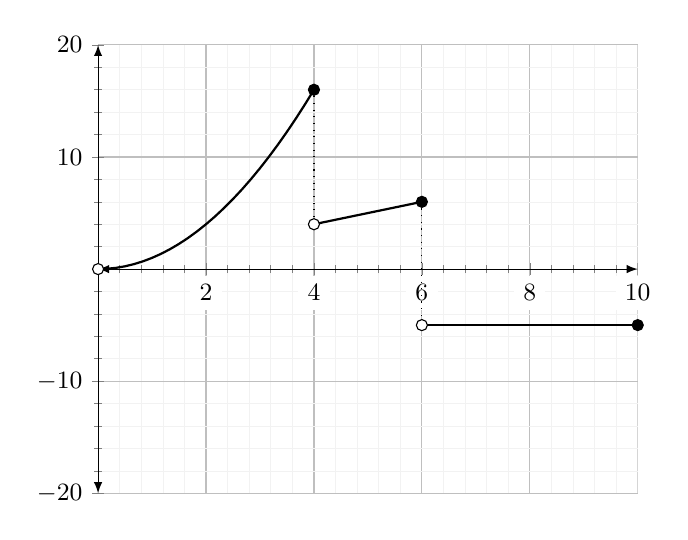
\begin{tikzpicture}[scale=1]
\begin{axis}[grid style={line width=.2pt, draw=gray!10},grid=both,major grid style={line width=.4pt,draw=gray!50},
    xmin=0,xmax=10,
    ymin=-20,ymax=20,
    xtick={},ytick={},
    minor tick num=4,
    enlargelimits={abs=0},
    ticklabel style={font=\small,fill=white},
    axis lines=middle,
    axis line style={latex-latex},
    xlabel style={at={(ticklabel* cs:1)},anchor=north west},
    ylabel style={at={(ticklabel* cs:1)},anchor=south west}
]
\addplot[domain=0:4,black, thick] {x*x};
\addplot[domain=4:6,black, thick] {x};
\addplot[domain=6:10,black, thick] {-5};
\draw[dotted] (axis cs:4,16) -- (axis cs:4,4);
\draw[dotted] (axis cs:6,6) -- (axis cs:6,-5);
\addplot[holdot] coordinates{(0,0)(4,4)(6,-5)};
\addplot[soldot] coordinates{(4,16)(6,6)(10,-5)};
\end{axis}
\end{tikzpicture}
& \quad &
\begin{enumerate}
\item$\d{\lim_{x \to 4^-} g(x) = \underline{\hspace{2cm}} }$
\item$\d{\lim_{x \to 4^+} g(x) = \underline{\hspace{2cm}} }$
\item$\d{\lim_{x \to 4} g(x) = \underline{\hspace{2cm}} }$
\item $g(4)= \underline{\hspace{2cm}}$
\item $\d{\lim_{x \to 8} g(x) = \underline{\hspace{2cm}} }$
\item $g(8)= \underline{\hspace{2cm}}$
\end{enumerate}
\end{tabular}

\item The function $h(x)$ is graphed below. Use the graph to fill in the blanks.

\begin{tabular}{m{9cm}  c m{5cm}}
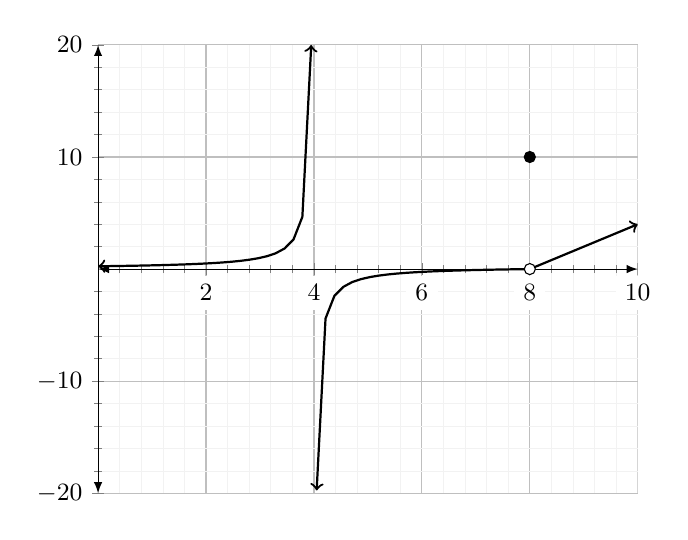
\begin{tikzpicture}[scale=1]
\begin{axis}[grid style={line width=.2pt, draw=gray!10},grid=both,major grid style={line width=.4pt,draw=gray!50},
    xmin=0,xmax=10,
    ymin=-20,ymax=20,
    xtick={},ytick={},
    minor tick num=4,
    enlargelimits={abs=0},
    ticklabel style={font=\small,fill=white},
    axis lines=middle,
    axis line style={latex-latex},
    xlabel style={at={(ticklabel* cs:1)},anchor=north west},
    ylabel style={at={(ticklabel* cs:1)},anchor=south west}
]

\addplot[<->,domain=0:3.95,black, thick] {(4-x)^(-1)};
\addplot[<-,domain=4.05:8,black, thick] {(4-x)^(-1)+0.25};
\addplot[->,domain=8:10,black, thick] {2*x-16};
%\draw[dotted] (axis cs:4,16) -- (axis cs:4,4);
%\draw[dotted] (axis cs:6,6) -- (axis cs:6,-5);
\addplot[soldot] coordinates{(8,10)};
\addplot[holdot] coordinates{(8,0)};
\end{axis}
\end{tikzpicture}
& \quad &
\begin{enumerate}
\item$\d{\lim_{x \to 4^-} h(x) = \underline{\hspace{2cm}} }$
\item$\d{\lim_{x \to 4^+} h(x) = \underline{\hspace{2cm}} }$
\item$\d{\lim_{x \to 4} h(x) = \underline{\hspace{2cm}} }$
\item $h(4)= \underline{\hspace{2cm}}$
\item $\d{\lim_{x \to 8} h(x) = \underline{\hspace{2cm}} }$
\item $h(8)= \underline{\hspace{2cm}}$
\end{enumerate}
\end{tabular}

\newpage
\item Find any vertical asymptotes of $f(x)=\frac{2}{x+5}$ and \emph{justify} your answer using a limit.
\vfill

\item Sketch the graph of an function that satisfies \emph{all} of the given conditions. Compare your answer with that of your neighbor.\\
\begin{tabular}{llll}
&&\\
$\displaystyle{\lim_{x \to 0^-} f(x)=1}$& $\displaystyle{\lim_{x \to 0^+ }f(x)=-2}$ &$\displaystyle{\lim_{x \to 4^-}f(x)=3}$&$\displaystyle{\lim_{x \to 4^+ }f(x)=0}$\\ 
&&\\
 $f(0)=-2$& &$f(4)=1$&\\
\end{tabular}
\vfill
\end{enumerate}
\end{document}

